\chapter{Su Kojo}
\begin{multicols}{2}
\section*{\color{black}Che cosa è Kojo?}
Kojo è una applicazione che può aiutare ad imparare a programmare un computer. Con Kojo si può scrivere del codice in un moderno ed estremamente potente linguaggio di programmazione {\bf\color{blue}Scala}. Kojo è Open Source ed è libero e disponibile per Linux, Windows e Mac.
\section*{\color{black}Dove posso trovare Kojo?}
Kojo può essere scaricato qui: 
\\

\href{http://www.kogics.net/kojo-download}{www.kogics.net/kojo-download}
\\

Per più informazioni: 
\\

\href{http://www.kogics.net/kojo}{www.kogics.net/kojo}

\columnbreak

\begin{center}
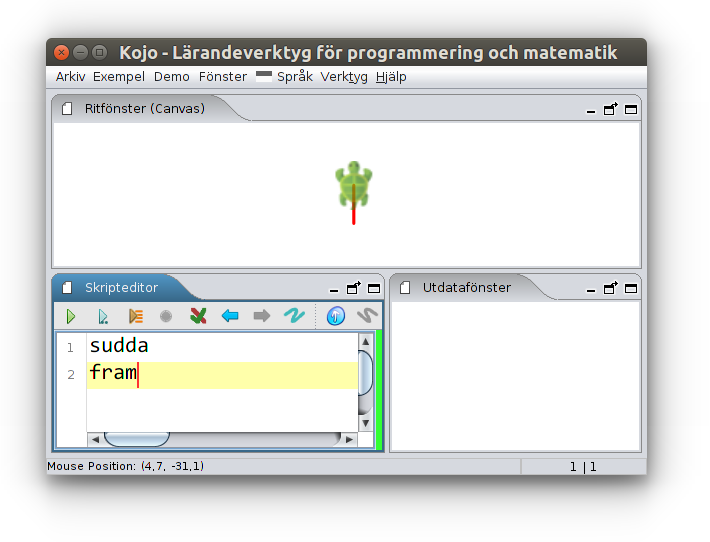
\includegraphics[width=14.0cm]{../img/kojo.png}
\end{center}

\end{multicols}

\chapter{Il vostro primo programma}
\begin{multicols}{2}
\section*{\color{BrickRed}Sfida:}
Scrivete quello che segue nell'area del codice:

\begin{lstlisting}[basicstyle={\ttfamily\fontsize{30}{36}\selectfont},numbers=none]
pulisci
avanti
\end{lstlisting}
        
Premete il bottone verde 

\includegraphics[width=1.0cm]{../img/play.png}
\\

per eseguire il codice.
\\

\vskip 5.0em

\columnbreak

\begin{center}
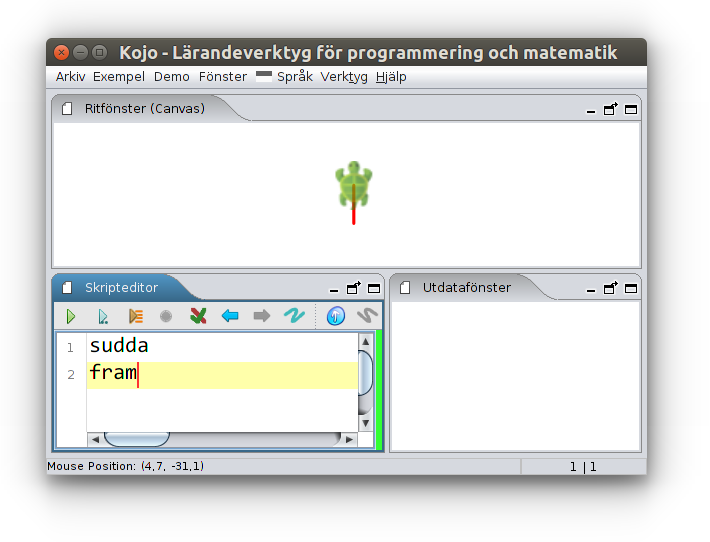
\includegraphics[width=14.0cm]{../img/fram.png}
\end{center}

\end{multicols}

\chapter{Disegnamo un quadrato}
\begin{multicols}{2}

\begin{lstlisting}[basicstyle={\ttfamily\fontsize{30}{36}\selectfont},numbers=none]
pulisci
avanti
destra
\end{lstlisting}
        
 Scrivendo \lstinline{sinistra} o \lstinline{destra} la tartaruga cambierà direzione.
\section*{\color{BrickRed}Sfida:}
Estendete il programma in moda da fare disegnare un quadrato.

\columnbreak

\begin{center}
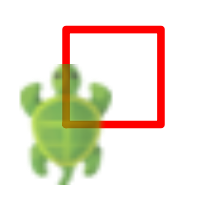
\includegraphics{../img/square.png}
\end{center}

\end{multicols}

\chapter{Disegnamo delle scale}
\begin{multicols}{2}

\begin{lstlisting}[basicstyle={\ttfamily\fontsize{30}{36}\selectfont},numbers=none]
pulisci
avanti; sinistra
avanti; destra
\end{lstlisting}
        
\vskip 1.0em
Con il punto e virgola \lstinline{;} tra le istruzioni, si possono avere più comandi sulla stessa linea.
\section*{\color{BrickRed}Sfida:}
Estendete il programma in maniera che disegni delle scale.

\columnbreak

\begin{center}
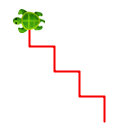
\includegraphics{../img/stairs.png}
\end{center}

\end{multicols}

\chapter{Facciamo un ciclo}
\begin{multicols}{2}

\begin{lstlisting}[basicstyle={\ttfamily\fontsize{30}{36}\selectfont},numbers=none]
pulisci
ripeti(4){ avanti; destra }
\end{lstlisting}
        
\section*{\color{BrickRed}Sfida:}


\begin{itemize}

\item {Cosa capiterà se cambiamo 4 in 100?}
\item {Disegnerà delle scale con 100 gradini.}

\end{itemize}



\columnbreak

\begin{center}
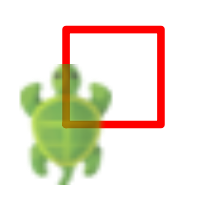
\includegraphics{../img/square.png}
\end{center}

\end{multicols}

\chapter{Disegnamo un personaggio}
\begin{multicols}{2}
\section*{\color{BrickRed}Sfida:}
Disegnate un personaggio di vostra scelta.
\section*{\color{OliveGreen}Tip:}

\begin{lstlisting}[basicstyle={\ttfamily\fontsize{20}{24}\selectfont},numbers=none]
salta
sinistra(180)
avanti(300)
salta(100)
saltaVerso(25,-28)
scrivi("FELIX is awesome")
colorePenna(purple)
coloreRiempimento(green)
\end{lstlisting}
        
Si può vedere la posizione della tartaruga in basso sulla sinistra mentre si muove il mouse sull'area di disegno:

\includegraphics[width=6.0cm]{../img/mousepos.png}


\columnbreak


\begin{center}
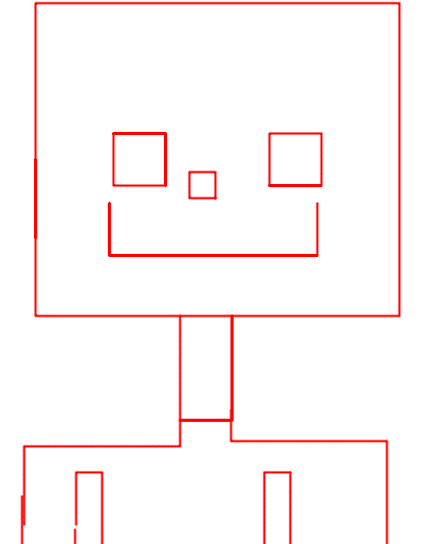
\includegraphics[width=4.5cm]{../img/man.png}
\end{center}

\vskip 2.0em
\begin{center}
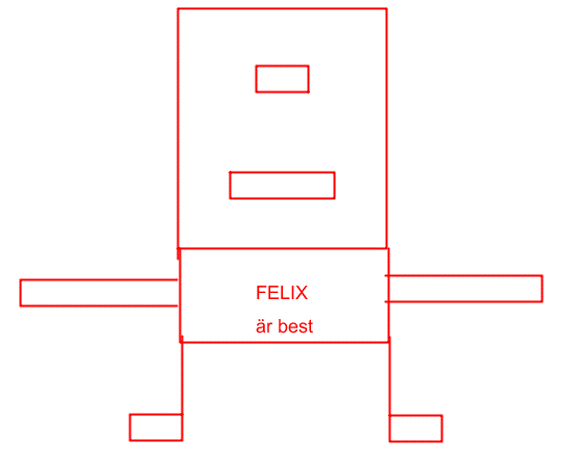
\includegraphics[width=9.0cm]{../img/alien.png}
\end{center}

\end{multicols}

\chapter{Quanto è veloce il vostro computer?}Il primo elaboratore elettronico era chiamato {\bf ENIAC} e poteva contare fino a 5000 in un secondo.\\
In Kojo c'è una funzione  \lstinline{räknaTill} che misura quanto veloce il vostro computer conti.\\
Eseguendo \lstinline{conta(5000)} sul mio computer più veloce, appare questa scritta nell'area di output:

\begin{lstlisting}[numbers=none]

*** 5000 *** PRONTO!
Ci sono voluti 0.32 millisecondi.
      
\end{lstlisting}
        
\section*{\color{BrickRed}Sfida:}


\begin{itemize}

\item {Eseguite \lstinline{conta(5000)} e controllate se il vostro computer è più veloce del mio.}
\item {Quando tempo tempo ci metterà il vostro computer a contare fino ad un milione?}
\item {Fino a che numero può contare in un secondo?}

\end{itemize}


\chapter{Tracciamo l'esecuzione del programma}
\begin{multicols}{2}
\section*{\color{BrickRed}Sfida:}


\begin{itemize}

\item {Scriviamo un programma che disegna scale.}
\item {Premiamo il bottone arancione.}
\item {Premiamo su uno dei comandi: \lstinline{CALL fram}. Cosa succede nell'area di disegno?}
\item {Quando una parte del codice è marcata in blu, solo quella parte verrà eseguita premendo il bottone di avvio. Possiamo deselezionare il codice facendo click dopo il codice che è selezionato. }
\item {Aggiungete altri comandi al vostro programma ed osservate cosa accade quando lo tracciate.}
\item {Chiudete la {\it Program trace} area quando avrete fatto.}

\end{itemize}



\columnbreak

\begin{center}
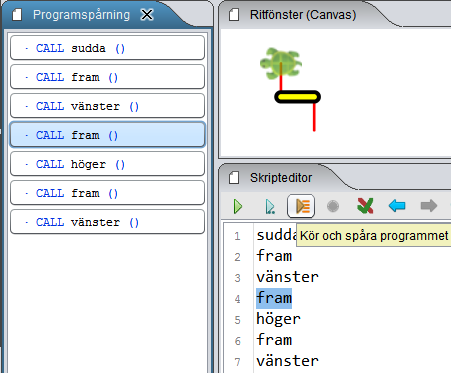
\includegraphics{../img/trace.png}
\end{center}

\end{multicols}

\chapter{Scriviamo le nostre funzioni con \lstinline{def}}Con \lstinline{def} si possono scrivere le proprie {\it funzioni} scegliendone il nome.

\begin{lstlisting}[basicstyle={\ttfamily\fontsize{20}{24}\selectfont},numbers=none]
def quadrato =  ripeti(4){ avanti; destra }  

pulisci
quadrato    //use your square-function
salta
quadrato
\end{lstlisting}
        
\section*{\color{BrickRed}Sfida:}


\begin{itemize}

\item {Cambiate il colore del quadrato.}
\item {Fatelo varie volte.}

\end{itemize}


\section*{\color{OliveGreen}Tip:}

\begin{lstlisting}[numbers=none]
coloreRiempimento(green); colorePenna(purple)
\end{lstlisting}
        
\chapter{Una pila di quadrati}
\begin{multicols}{2}
\section*{\color{BrickRed}Sfida:}
Facciamo una pila di 10 quadrati
\section*{\color{OliveGreen}Tip:}
\vskip 1.0em

\begin{lstlisting}[numbers=none]
def quadrato =  ripeti(4){ avanti; destra }  

pulisci; ritardo(100)
ripeti(10){ ??? }
\end{lstlisting}
        

\columnbreak

\begin{center}
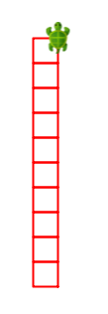
\includegraphics{../img/square-column.png}
\end{center}

\end{multicols}

\chapter{Una funzione per fare le pile}
\begin{multicols}{2}
\section*{\color{BrickRed}Sfida:}
Scrivete una funzione chiamata \lstinline{pila}, che disegna una pila di 10 quadrati.
\section*{\color{OliveGreen}Tip:}

\begin{lstlisting}[numbers=none]
def quadrato = ripeti(4){ avanti; destra }  
def pila = ???

pulisci; ritardo(100)
pila
\end{lstlisting}
        

\columnbreak

\begin{center}
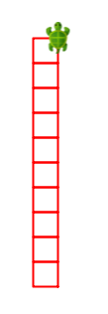
\includegraphics{../img/square-column.png}
\end{center}

\end{multicols}

\chapter{Facciamo una griglia}
\begin{multicols}{2}
\section*{\color{BrickRed}Sfida:}
Fate una griglia 10*10 di quadrati.
\section*{\color{OliveGreen}Tip:}


\begin{itemize}

\item {Usate la vostra funzione per le pile (stack) che avete scritto prima.}
\item {Saltate indietro di una inter colonna con \lstinline{salta(-10 * 25)}}
\item {Saltate nella giusta posizione con \lstinline{destra; salta; destra}}

\end{itemize}



\columnbreak

\begin{center}
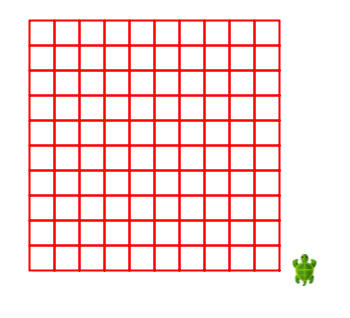
\includegraphics{../img/square-grid.png}
\end{center}

\end{multicols}

\chapter{Un quadrato parametrico}
\begin{multicols}{2}
\section*{\color{BrickRed}Sfida:}
DIsegnamo un quadrato di dimensioni differenti.
\section*{\color{OliveGreen}Tip:}
Date alla vostra funzione un {\it parameter},\\
chiamato \lstinline{side} di tipo \lstinline{Int}:

\begin{lstlisting}[basicstyle={\ttfamily\fontsize{16}{19}\selectfont},numbers=none]
def quadrato(side : Int) = 
  ripeti(4){ avanti(side); destra }

pulisci; ritardo(100); invisibile
quadrato(100) 
quadrato(70)
quadrato(40)
\end{lstlisting}
        
Potete cambiare il colore con:\\
\lstinline{coloreRiempimento(blue); colorePenna(pink)}


\columnbreak


\begin{center}
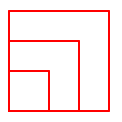
\includegraphics[width=5.0cm]{../img/square-param.png}
\end{center}

\begin{center}
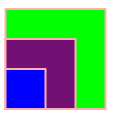
\includegraphics[width=5.0cm]{../img/square-param-color.png}
\end{center}

\end{multicols}

\chapter{Disegnamo un personaggio a quadrati}\section*{\color{BrickRed}Sfida:}
Disegnate un personaggio con quadrati di dimensione differente.
\\


\begin{tikzpicture}[overlay]
\node at (20.0cm,-1.0cm) {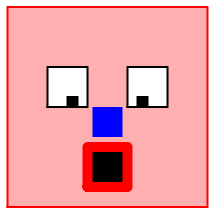
\includegraphics[width=5.5cm]{../img/square-man.png}};
\end{tikzpicture}
  
\section*{\color{OliveGreen}Tip:}

\begin{lstlisting}[basicstyle={\ttfamily\fontsize{14}{17}\selectfont},numbers=none]
def quadrato(x: Int, y: Int, side: Int) = {
  saltaVerso(x, y)
  ripeti(4) { avanti(side); destra }
}
def testa(x: Int, y: Int)  = { coloreRiempimento(pink); colorePenna(red); quadrato(x, y, 200) }
def occhio(x: Int, y: Int)   = { coloreRiempimento(white); colorePenna(black); quadrato(x, y, 40) }
def pupilla(x: Int, y: Int) = { coloreRiempimento(black); colorePenna(black); quadrato(x, y, 10) }
def naso(x: Int, y: Int)  = { coloreRiempimento(blue); colorePenna(noColor); quadrato(x, y, 30) }
def bocca(x: Int, y: Int) = { impostaSpessorePenna(10); coloreRiempimento(black); colorePenna(red); quadrato(x, y, 40) }

pulisci; ritardo(20); invisibile
testa(0, 0)
occhio(40, 100); pupilla(60, 100)
???
\end{lstlisting}
        
\chapter{Disegnamo un poligono}\section*{\color{BrickRed}Sfida:}


\begin{itemize}

\item {Provate il codice qui sotto. DIsegnate diversi tipi di poligoni.}
\item {Aggiungete un parametro \lstinline{side} e disegnate dei poligoni di dimensioni differenti.}
\item {Quanto dovrebbe essere largo n per farlo sempreare un cerchio?}

\end{itemize}


\section*{\color{OliveGreen}Tip:}

\begin{lstlisting}[basicstyle={\ttfamily\fontsize{18}{22}\selectfont},numbers=none]
def poligono(n:Int) = ripeti(n){
  avanti(100)
  sinistra(360.0/n)
}

pulisci; ritardo(100)
poligono(7)
\end{lstlisting}
        

\begin{tikzpicture}[overlay]
\node at (20.0cm,3.5cm) {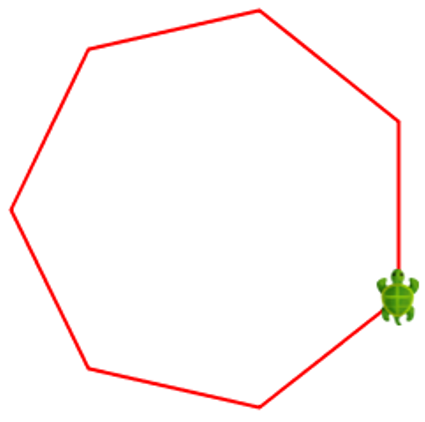
\includegraphics[width=8.0cm]{../img/polygon.png}};
\end{tikzpicture}
  
\chapter{Disegnamo alcuni poligoni}\section*{\color{BrickRed}Sfida:}


\begin{itemize}

\item {Provate il codice qui sotto.}
\item {Cercate di cambiare il numero di lati e di angoli.}
\item {Colorate i poligoni in colori differenti.}

\end{itemize}



\begin{tikzpicture}[overlay]
\node at (22.0cm,-0.5cm) {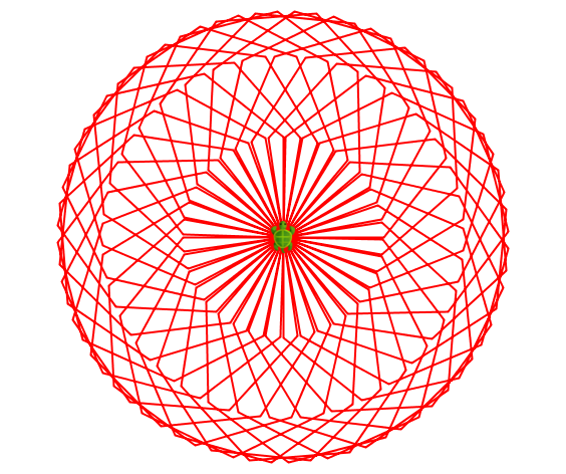
\includegraphics[width=11.0cm]{../img/polygons-circle.png}};
\end{tikzpicture}
  

\begin{lstlisting}[basicstyle={\ttfamily\fontsize{16}{19}\selectfont},numbers=none]
def poligono(n: Int, side: Int) = ripeti(n){
  avanti(side)
  sinistra(360.0/n)
}
def ruota(n: Int, heading: Int, side: Int) = 
  ripeti(360/heading){ poligono(n, side); sinistra(heading) }

pulisci; ritardo(5)
ruota(7, 10, 100)
\end{lstlisting}
        
\chapter{Valori ed espressioni}
\begin{multicols}{2}
\section*{\color{BrickRed}Sfida:}


\begin{itemize}

\item {Scrivete \lstinline{1 + 1} e premete il bottone blu. Kojo creerà un commento verde.}
\item {Il commento mostra il valore dell'espressione \lstinline{1 + 1} che è equivalente a \lstinline{2} ed il cui tipo è \lstinline{Int}, che significa numero intero.}
\item {Scrivete altre espressioni. Che valori e che tipi hanno le espressioni qui sotto?}

\end{itemize}



\begin{lstlisting}[numbers=none]
5 * 5
10 + 2 * 5
"Hello" + "world"
5 / 2
5 / 2.0
5 % 2
\end{lstlisting}
        


\columnbreak


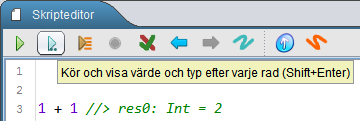
\includegraphics[width=12.0cm]{../img/show-value.png}
\section*{\color{OliveGreen}Tip:}


\begin{itemize}

\item {\lstinline{/} tra numeri interi la divisione ignora i valori decimali (divisione intera). Per essere sicuri che la divisione non sia di tipo intero uno dei due operandi deve avere numeri decimali. Il tipo di un numero decimale è chiamato \lstinline{Double}.}
\item {Con \lstinline{%} si può avere il resto di una divisione intera.}

\end{itemize}


\end{multicols}

\chapter{Diamo un nome ad un valore con \lstinline{val}}
\begin{multicols}{2}
\section*{\color{BrickRed}Sfida:}
Con \lstinline{val} si può riferire un nome ad un valore. Si può usare il nome al posto del valore. Provate il programma sotto. Cosa scriverà la tartaruga?

\begin{lstlisting}[numbers=none]
val x = 10
val y = 5
val cocomero = x + y
val banana = x * y

pulisci
avanti; scrivi(banana)
avanti; scrivi(cocomero)
avanti; scrivi(y)
avanti; scrivi(x)
\end{lstlisting}
        

\columnbreak

\begin{center}
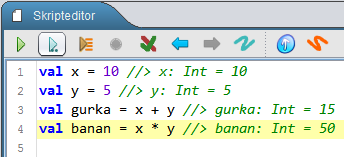
\includegraphics[width=12.0cm]{../img/val.png}
\end{center}

\end{multicols}

\chapter{Numeri casuali}\section*{\color{BrickRed}Sfida:}


\begin{itemize}

\item {Fate eseguire il programma sotto varie volte, cose succede?}
\item {Quale è il più piccolo ed il più grande valore possibile del raggio \lstinline{r}?}
\item {Cambiate il raggio così che \lstinline{r} diventi un numero casuale compreso tra 3 e 200.}
\item {Disegnate 100 cerchi, ognuno con un raggio casuale ad una posizione casuale come mostrato nella figura.}

\end{itemize}



\begin{tikzpicture}[overlay]
\node at (21.0cm,-5.0cm) {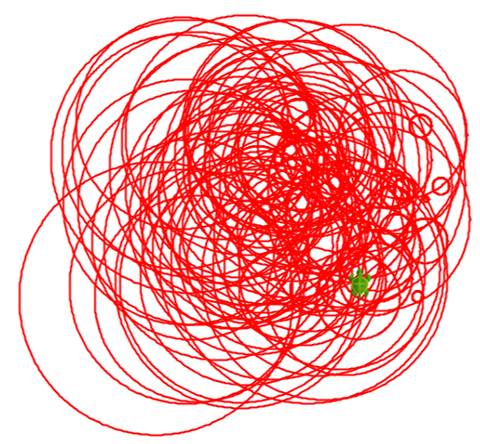
\includegraphics[width=8.0cm]{../img/random-circles.png}};
\end{tikzpicture}
  

\begin{lstlisting}[basicstyle={\ttfamily\fontsize{20}{24}\selectfont},numbers=none]
//r becomes a random number between 10 and 99:
val r = numeroCasuale(90) + 10   

pulisci; ritardo(10); invisibile
scrivi("Radius = " + r)
cerchio(r)
\end{lstlisting}
        
\chapter{Misceliamo i nostri colori}

\begin{itemize}

\item {Potete mischiare i vostri colori con \lstinline{Color}, per esempio \lstinline{Color(0, 70, 0)}}
\item {I tre parametri sono i valori per {\it red}, {\it green} e {\it blue}}
\item {Potete aggiungere un quarto parametro che imposterà la {\it transparency}}
\item {L'intervallo per i parametri è un numero intero compreso tra 0 e 255}

\end{itemize}


\section*{\color{BrickRed}Sfida:}
Provate il programma sotto e cambiate la trasparenza del colore

\begin{tikzpicture}[overlay]
\node at (23.0cm,-2.0cm) {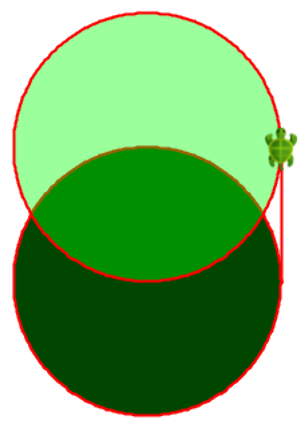
\includegraphics[width=7.0cm]{../img/color-circles.png}};
\end{tikzpicture}
  

\begin{lstlisting}[basicstyle={\ttfamily\fontsize{16}{19}\selectfont},numbers=none]
pulisci; ritardo(100)      

val verdeOliva = Color(0,70,0)
val pistacchio = Color(0,255,0,100)

coloreRiempimento(verdeOliva); cerchio(100)
coloreRiempimento(pistacchio); avanti(100); cerchio(100)
\end{lstlisting}
        
\chapter{Proviamo il selettore dei colori}
\begin{multicols}{2}
\section*{\color{BrickRed}Sfida:}


\begin{itemize}

\item {Fate click con il tasto destro del mouse nell'area del codice e selezionate \lstinline{Choose color...}}
\item {Se scegliete la linguetta {\bf RGB} potrete scegliere un nuovo colore in valori RGB.}
\item {Premete Ok e guardate nell'area di output. Potrete notare i valori RGB pe il rosso, il verde ed il blu.}
\item {Potete usare questi valori nei vostri programmi per disegnare con il vostro nuovo colore, per esempio in questo modo: \lstinline{colore(Color(218,153,67))}.}

\end{itemize}



\columnbreak

\begin{center}
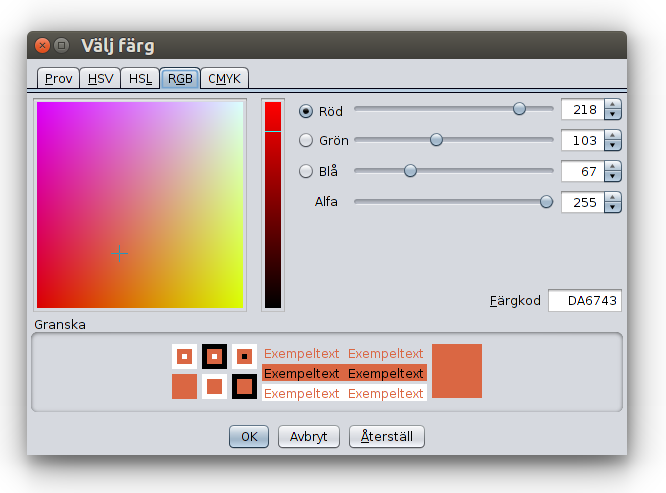
\includegraphics[width=14.0cm]{../img/color-chooser-rgb-sv.png}
\end{center}

\end{multicols}

\chapter{Disegnamo dei cerchi casuali}
\begin{multicols}{2}

\begin{lstlisting}[basicstyle={\ttfamily\fontsize{16}{19}\selectfont},numbers=none]
def random = numeroCasuale(256)
def randomColor = Color(random,10,random,100) 

pulisci; numeroCasuale(5)
gradiente(black,white)
impostaSpessorePenna (6)

ripeti(100) {
    colorePenna(randomColor)
    cerchio(100)
    salta(20)
    destra(35)
}
\end{lstlisting}
        
\section*{\color{BrickRed}Sfida:}
Provate differenti colori e sfondi casuali.


\columnbreak


\begin{center}
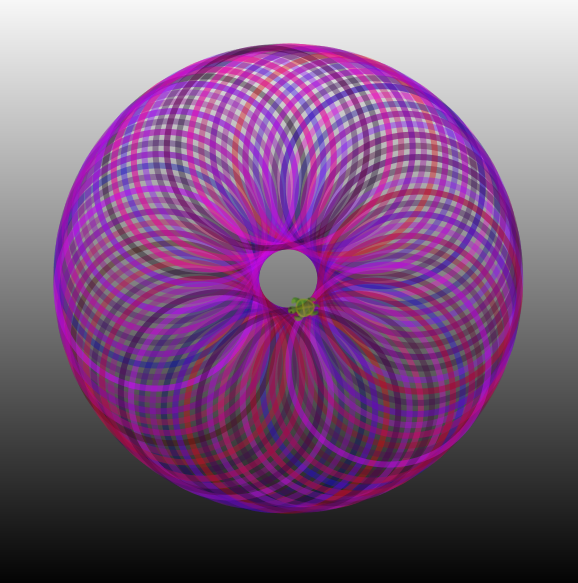
\includegraphics[width=12.0cm]{../img/circle-of-circles.png}
\end{center}

\end{multicols}

\chapter{Disegnamo un fiore}\section*{\color{BrickRed}Sfida:}
Il programma qui sotto disegna 100 cerchi colorati casualmente, ognuno con posizione e raggio casuale. Cambiate i parametri e cercate di spiegare che succede.

\begin{tikzpicture}[overlay]
\node at (22.0cm,-4.0cm) {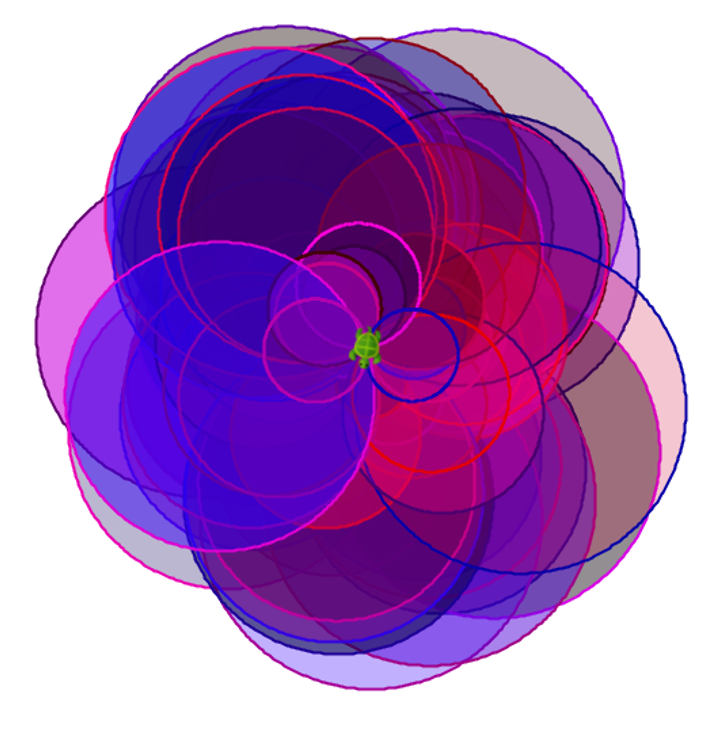
\includegraphics[width=8.5cm]{../img/random-color-circles.png}};
\end{tikzpicture}
  

\begin{lstlisting}[basicstyle={\ttfamily\fontsize{16}{19}\selectfont},numbers=none]
pulisci(); ritardo(5)
impostaSpessorePenna (2)
ripeti(100){
  colorePenna(Color(random(256),0,random(256)))
  coloreRiempimento(Color(random(256),0,random(256),random(100)+50))
  sinistra(random(360))
  cerchio(random(30)*4+10)
}
\end{lstlisting}
        
\chapter{Creiamo una variabile con \lstinline{var}}Con \lstinline{var} si può associare un nome ad un valore, ma questo può essere cambiato in seguito.\\
Potete prendere la variabile ed assegnargli un valore in questo modo:

\begin{lstlisting}[numbers=none]

var cucumber = 1
cucumber = 1 + 1   //first calculate 1 + 1 and then assign that number to cucumber     
        
\end{lstlisting}
        
\section*{\color{BrickRed}Sfida:}
Provate questo programma. Cosa scriverà la tartaruga?

\begin{lstlisting}[basicstyle={\ttfamily\fontsize{16}{19}\selectfont},numbers=none]
var i = 0

pulisci
ripeti(10){
  i = i + 1
  avanti; scrivi(i)
}
\end{lstlisting}
        
\section*{\color{OliveGreen}Tip:}


\begin{itemize}

\item {Nella espressione \lstinline{i = i + 1} ad \lstinline{i} è stato assegnato il {\it old} valore di \lstinline{i} più \lstinline{1}}

\end{itemize}


\chapter{Disegnamo alcuni fiori}\section*{\color{BrickRed}Sfida:}


\begin{itemize}

\item {Fate una funzione chiamata \lstinline{flower}, che disegna una corolla da cui parte un ramo con una foglia verde.}
\item {Disegnate 5 fiori uno accanto all'altro.}

\end{itemize}



\begin{tikzpicture}[overlay]
\node at (15.0cm,-7.0cm) {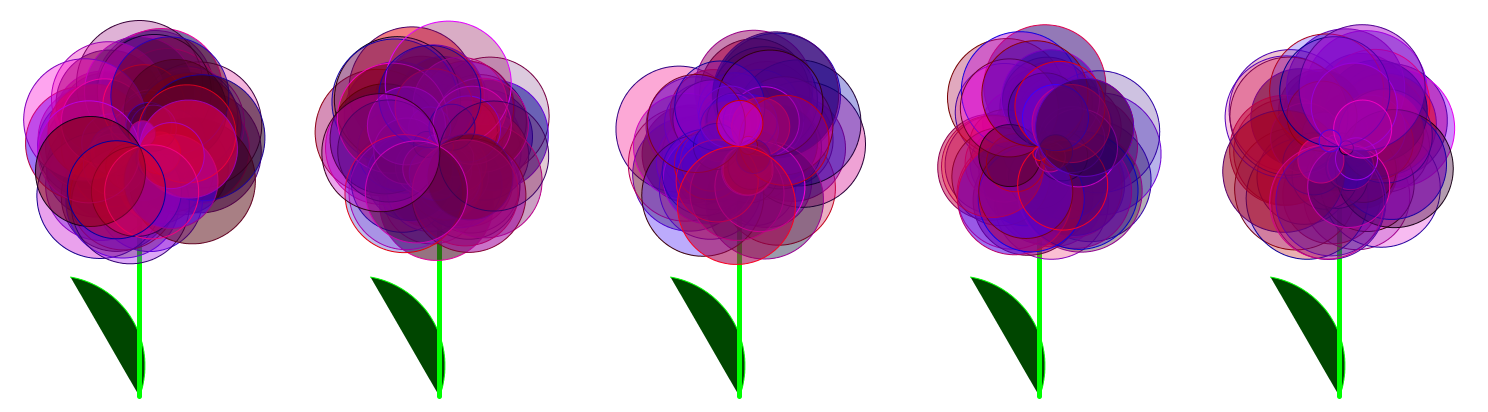
\includegraphics[width=16.0cm]{../img/flowers.png}};
\end{tikzpicture}
  
\section*{\color{OliveGreen}Tip:}
Potete disegnare le foglie con \lstinline{arco(radius, angle)}. \\
Fate che la funzione \lstinline{fiore.} abbia due parametri, x e y, e usate \lstinline{saltaVerso(x,y)}\\
Potete ripetere il ciclo 5 volte e calcolare la posizione in questo modo:

\begin{lstlisting}[basicstyle={\ttfamily\fontsize{18}{22}\selectfont},numbers=none]
var i = 0          
ripeti(5){
  fiore(600*i,0)
  i = i + 1        
}
\end{lstlisting}
        
\chapter{Cambiamo l'immagine della tartaruga}\section*{\color{BrickRed}Sfida:}
Scaricate i file aggiuntivi dalla pagin web di Kojos:
\href{http://www.kogics.net/kojo-download#media}{www.kogics.net/kojo-download\#media}


\begin{itemize}

\item {Decomprimete il file \lstinline{scratch-media.zip} e cercate l'immagine del granchio \lstinline{crab1-b.png} nella cartella \lstinline{Media/Costumes/Animals}}
\item {Posizionate il file \lstinline{crab1-b.png} nella stessa cartella del programma.}
\item {Cercate di cambiare l'immagine della tartaruga in un granchio in questo modo:}

\end{itemize}



\begin{tikzpicture}[overlay]
\node at (12.0cm,-2.5cm) {
\includegraphics[width=4.0cm]{../img/crab1-b.png}};
\end{tikzpicture}
  

\begin{lstlisting}[basicstyle={\ttfamily\fontsize{20}{24}\selectfont},numbers=none]
pulisci
indossaCostume ("crab1-b.png")  
ritardo(2000)
avanti(1000)
\end{lstlisting}
        
\section*{\color{OliveGreen}Tip:}


\begin{itemize}

\item {Potete usare anche delle vostre immagini, basta che siano del tipo \lstinline{.png} o \lstinline{.jpg}}
\item {Se volte mettere le immagini in una cartella diversa da quella del programma, dovrete fornire il percorso sul disco rigido dove poter rintracciare il file, per esempio \lstinline{indossaCostume("~/Kojo/Media/Costumes/Animals/crab1-b.png")} dove \lstinline{~} significa la vostra cartella personale (la cartella home per i sistemi operativi di tipo Unix).}

\end{itemize}


\chapter{Facciamo una nuova tartaruga con \lstinline{new}}Potere creare altre tartarughe con il comando \lstinline{new} in questo modo:

\begin{lstlisting}[basicstyle={\ttfamily\fontsize{18}{22}\selectfont},numbers=none]
pulisci
val p1 = new Tartaruga(100,100) //the new turtle p1 starts on position (100, 100)
val p2 = new Tartaruga(100, 50)  //the new turtle p2 starts on position (100, 50)
p1.avanti(100)
p2.avanti(-100)  //turtle p2 backs up
\end{lstlisting}
        

\begin{tikzpicture}[overlay]
\node at (22.0cm,-2.0cm) {
\includegraphics[width=5.0cm]{../img/new.png}};
\end{tikzpicture}
  
\section*{\color{BrickRed}Sfida:}


\begin{itemize}

\item {Create tre tartarughe che siano posizionate una vicino all'altra.}
\item {Fatele girare verso sinistra.}

\end{itemize}


\section*{\color{OliveGreen}Tip:}


\begin{itemize}

\item {\lstinline{p1} e \lstinline{p2} sono i {\it names} delle tartarughe. Potete farne quante volete.}
\item {Con il nome \lstinline{p1} ed un punto, potete dare alle specifiche tartarughe dei comandi, per esempio così: \lstinline{p1.sinistra}}
\item {\lstinline{invisibile} nasconde le tartarughe.}

\end{itemize}


\chapter{Una corsa di tartarughe}
\begin{multicols}{2}
Con l'aiuto dei numeri casuale potrete programmare una corsa di tartarughe.
\section*{\color{BrickRed}Sfida:}


\begin{itemize}

\item {Impostate una corsa tra tre tartarughe.}
\item {Fate che corrano in avanti per 10 volte. Quale vincerà?}

\end{itemize}


\section*{\color{OliveGreen}Tip:}


\begin{itemize}

\item {Con \lstinline{p1.avanti(random(100) + 1)} la tartaruga p1 muoverà da 1 a 100 passi in avanti}

\end{itemize}



\columnbreak

\begin{center}
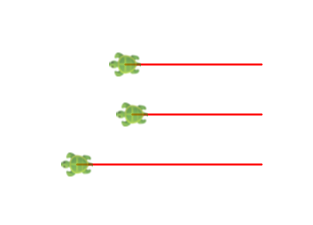
\includegraphics[width=12.0cm]{../img/race.png}
\end{center}

\end{multicols}

\chapter{Le scelte alternative con \lstinline{if}}Con una istruzione \lstinline{if} il computer sceglierà una delle due differenti alternative in dipendenza da una condizione che può risultare vera o falsa.

\begin{lstlisting}[basicstyle={\ttfamily\fontsize{20}{24}\selectfont},numbers=none]
pulisci; invisibile
if (true) scrivi("true") else scrivi("false")
\end{lstlisting}
        
\section*{\color{BrickRed}Sfida:}


\begin{itemize}

\item {Cambiate \lstinline{true} in \lstinline{false} e controllate cosa scrive la tartaruga.}
\item {Cambiate la condizione in \lstinline{2 > 1} e controllate cosa scrive la tartaruga.}
\item {Cambiate la condizione in \lstinline{2 < 1} e controllate cosa scrive la tartaruga.}
\item {Spiegate come l'espressione \lstinline{if} funziona.}

\end{itemize}


\section*{\color{OliveGreen}Tip:}


\begin{itemize}

\item {Se la condizione dopo \lstinline{if} è \lstinline{true} viene preso quello subito dopo.}
\item {Se la condizione dopo \lstinline{if} è \lstinline{false} viene preso quello dopo \lstinline{else}.}

\end{itemize}


\chapter{Reagire a quello che l'utente sta facendo}
\begin{lstlisting}[basicstyle={\ttfamily\fontsize{20}{24}\selectfont},numbers=none]
pulisciOutput; setOutputTextFontSize(35)
val password = "cocomero"
val question     = "What is the password?"
val right      = "The safe is open!"
val wrong       = "You may not come in!"
val answer = leggi(answer)  //wait for an answer from the user
val message = if (answer == password) right else wrong
scriviLinea(message)
\end{lstlisting}
        
\section*{\color{BrickRed}Sfida:}


\begin{itemize}

\item {Eseguire il programma e spiegare cosa stia facendo.}
\item {Cambiare la password, la domanda e cosa è stampato quando la risposta è giusta o sbagliata.}
\item {Chiedere anche il nome dell'utente ed aggiungerlo a quello che viene scritto.}

\end{itemize}


\chapter{Facciamo un ciclo \lstinline{while}}Con il ciclo while \lstinline{while} il computer ripeterà un comando tante volte finché la condizione sarà vera.

\begin{lstlisting}[basicstyle={\ttfamily\fontsize{22}{27}\selectfont},numbers=none]
pulisci; invisibile; ritardo(250); pulisciOutput
var x = 200
while (x > 0) {  //check the condition before each round 
  avanti(x); destra
  scrivi(x) 
  x = x - 12
}
scriviLinea("x is now: " + x)
\end{lstlisting}
        
\section*{\color{BrickRed}Sfida:}


\begin{itemize}

\item {Cosa viene scritto nell'area di output? Perché?}
\item {Tracciate il programma con il bottone arancione di esecuzione e controllate ogni passo.}
\item {Cambiate la riduzione di \lstinline{x} da \lstinline{12} a \lstinline{20}. Spiegate cosa succede.}

\end{itemize}


\chapter{Indovina il numero}
\begin{lstlisting}[basicstyle={\ttfamily\fontsize{16}{19}\selectfont},numbers=none]
val secretNumber = numeroCasuale(100)+1
var answer = leggiLinea("Guess a number between 1 and 100! ")
var continue = true

while (continue) {
    if (answer.toInt < secretNumber)
      answer = leggiLinea(answer + " is too SMALL, guess again!")
    else if (answer.toInt > secretNumber)
      answer = leggiLinea(answer + " is too LARGE, guess again!")
    else if (answer.toInt == secretNumber)
      continue = false
}
scriviLinea(secretNumber + " is the CORRECT answer!")
\end{lstlisting}
        
\section*{\color{BrickRed}Sfida:}
Introducete una variabile \lstinline{var numberOfTries = 0} e contate ad ogni tentativo.\\
Quando pronti scrivete il numero dei tentativi in questo modo:\\
\lstinline{Correct answer! You got it in 5 guesses}
\chapter{Fare pratica nella moltiplicazione}
\begin{lstlisting}[basicstyle={\ttfamily\fontsize{16}{19}\selectfont},numbers=none]
var rightAnswers = 0
val startTime = System.currentTimeMillis / 1000
ripeti(12) {
  val number1 = numeroCasuale(12)+1
  val number2 = numeroCasuale(12)+1
  val answer = leggiLinea("What is  " + number1 + "*" + number2 + "?")
  if (answer == (number1 * number2).toString) {
    scriviLinea("Correct!")
    rightAnswers = rightAnswers + 1
  }
  else scriviLinea("Wrong. The right answer is " + (number1 * number2))
}
val stopTime = System.currentTimeMillis / 1000
val sec = stopTime - startTime
scriviLinea("You got " + rightAnswers + " right answer in " + sec + " seconds")
\end{lstlisting}
        
\section*{\color{BrickRed}Sfida:}
Cambiate per poter fare pratica solo nella moltiplicazione con 8 e 9.
\chapter{Immagazzinare gli animali in una lista}
\begin{lstlisting}[basicstyle={\ttfamily\fontsize{14}{17}\selectfont},numbers=none]
var animal = Vector("elk", "cow", "rabbit", "mite")  // the variable animal refers to a vector with 4 animals
scriviLinea("The first animal in the vector is: " + animal(0))     //the positions in a vector are counted from 0
scriviLinea("The second animal in the vector is:  " + animal(1))
scriviLinea("There are these many animals in the vector: " + animal.size)
scriviLinea("The last animal in the vector is:  " + animal(animal.size-1))

val s = numeroCasuale(animal.size)   //take a random number between 0 and the number of animals minus 1
scriviLinea("A random animal: " + animal(s))
animal = animal :+ "camel"    //adds another animal last in the vector
animal = "dromedary" +: animal // adds another animal first in the vector

animal = animal.updated(2, "mudskipper")  // Change the third animal(index 2 in vector)
scriviLinea("All animals in the array backwards:")
animal.foreach{ x => scriviLinea(x.reverse) } // for all x in array: type out x backwards.
\end{lstlisting}
        
\section*{\color{BrickRed}Sfida:}


\begin{itemize}

\item {Cosa stampera il programma nell'area di output? Spiegate cosa succede.}
\item {Aggiungete altri animali alla lista.}

\end{itemize}


\chapter{Fare pratica nelle parole}
\begin{lstlisting}[basicstyle={\ttfamily\fontsize{14}{17}\selectfont},numbers=none]
val Swedish = Vector("dator", "sköldpadda", "cirkel")
val English = Vector("computer", "turtle", "circle")
var amountRight = 0
ripeti(5) {
  val s = numeroCasuale(3)
  val word = Swedish(s)
  val answer = leggiLinea("What is " + word + " in English?")
  if (answer == English(s)) {
    scriviLinea("Correct answer!")
    amountRight = amountRight + 1
  } else {
    scriviLinea("Wrong answer. Correct answer is: " + English(s))
  }
}
scriviLinea("You have" + amountRight + " correct answers.")
\end{lstlisting}
        
\section*{\color{BrickRed}Sfida:}


\begin{itemize}

\item {Aggiungete altre parole.}
\item {Fare pratica nelle parole dall'inglese all'italiano.}
\item {Fate scegliere più domande prima di finire. Suggerimento: \lstinline{val amount = input("Amount: ").toInt} }

\end{itemize}


\chapter{Il gioco delle Capitali}
\begin{lstlisting}[basicstyle={\ttfamily\fontsize{13}{16}\selectfont},numbers=none]
def capitalGame = {
  scriviLinea("Welcome to the Capital Game!")
  val city = Map("Sweden" ->"Stockholm", "Denmark" -> "Copenhagen", "Skåne" -> "Malmö")
  var countriesLeft = city.keySet //keySet gives an amount of all keys in a Map 
  def randomCountry = scala.util.Random.shuffle(countriesLeft.toVector).head
  while(!countriesLeft.isEmpty) {
    val country = randomCountry
    val answer = input("What is the capital in " + country + "?")
    output(s"You wrote: $answer")
    if (answer == city(country)) {
      output("Correct answer! You have " + countriesLeft.size + " countries left!")
      countriesLeft = countriesLeft - country  //remove country from the set of countries left
    } else output(s"Wrong answer. The capital in $country begins with ${city(country).take(2)}...")
  }
  output("THANK YOU FOR PLAYING! (Press ESC)")
}

toggleFullScreenOutput;  
setOutputBackground(black); setOutputTextColor(green); setOutputTextFontSize(30)
ripeti(100)(output("")) //scroll the output window with 100 blank rows.
capitalGame

// *** TASK: (1) Add more pairs of countries and cities: country -> city (2) Measure time and count points.
\end{lstlisting}
        
\chapter{Fare un timer con \lstinline{object}}
\begin{lstlisting}[basicstyle={\ttfamily\fontsize{14}{17}\selectfont},numbers=none]
object timer {
  def now = System.currentTimeMillis  //gives time now in milliseconds.
  var time = now
  def reset = { time = now }
  def measure = now - time
  def randomWait(min: Int, max: Int) =  //wait between min and max seconds
    Thread.sleep((numeroCasuale(max-min)+min)*1000)  //Thread.sleep(1000) waits 1 second
}

println("Click in the println window and wait...")
timer.randomWait(3,6)   //wait between 3 and 6 seconds
timer.reset
readln("Press Enter as fast as you can.")
println("Reaction time: " + (timer.measure/1000.0) + " seconds")
\end{lstlisting}
        
Con \lstinline{object} è possibile raccogliere cose che sono in relazione tra loro in un oggetto.\\
Potete raggiungere una cosa all'interno di un oggetto con un punto: \lstinline{timer.reset}
\section*{\color{BrickRed}Sfida:}


\begin{itemize}

\item {Provate il programma e misurate il tempo di reazione. Quanto siete veloci?}
\item {Usate \lstinline{timer} nel compito {\it Guess the number} ed aggiungete un modo per scrivere: \lstinline{Correct answer! You made it in 5 guesses and 32 seconds}}

\end{itemize}


\chapter{Simulazione di un semaforo}
\begin{tikzpicture}[overlay]
\node at (22.0cm,-6.0cm) {
\includegraphics[width=3.0cm]{../img/traffic-lights.png}};
\end{tikzpicture}
  

\begin{lstlisting}[basicstyle={\ttfamily\fontsize{14}{17}\selectfont},numbers=none]
def turnOffAll = draw(penColor(gray) * fillColor(black) -> PicShape.rect(130,40))
def light(c: Color, h: Int) = penColor(noColor) * fillColor(c) * trans(20,h) -> PicShape.circle(15)
def lightRed = draw(light(red, 100))
def lightYellow = draw(light(yellow, 65))
def lightGreen = draw(light(green, 30))
def wait(seconds: Int) = Thread.sleep(seconds*1000)

pulisci; invisibile  
while (true) { //an infinite loop
  turnOffAll
  lightRed;  wait(3)
  lightYellow;  wait(1) 
  turnOffAll
  lightGreen; wait(3)
  lightYellow;  wait(1)
}
\end{lstlisting}
        
\section*{\color{BrickRed}Sfida:}


\begin{itemize}

\item {Cosa succede quando il semaforo cambia colore? Cercate di spiegare cosa succede.}
\item {Fate una modifica in modo che la luce verde sia accesa per il doppio del tempo.}

\end{itemize}


\chapter{Controllare la tartaruga con la tastiera}
\begin{multicols}{2}

\begin{lstlisting}[basicstyle={\ttfamily\fontsize{18}{22}\selectfont},numbers=none]
pulisci; ritardo(0)
activateCanvas()

animate { avanti(1) }

onKeyPress { k =>
  k match {
    case Kc.VK_LEFT =>   sinistra(5)
    case Kc.VK_RIGHT =>  destra(5)
    case Kc.VK_SPACE =>  avanti(5)
    case _ => 
      scriviLinea("Another key: " + k)
  }
}
\end{lstlisting}
        


\columnbreak


\section*{\color{BrickRed}Sfida:}


\begin{itemize}

\item {Scrivete \lstinline{Kc.} e premete \lstinline{Ctrl+Alt+Space} e guardate i diversi tasti premuti.}
\item {Chiamare \lstinline{alzaPenna} premento freccia su}
\item {Chiamare \lstinline{abbassaPenna} premento freccia giù}
\item {FaChiamarete \lstinline{color(blue)} premendo il tasto B}
\item {Chiamare \lstinline{color(red)} premendo il tasto R}
\item {Aumentare o diminuire la velocità premendo + o -}

\end{itemize}


\end{multicols}

\chapter{Controllare la tartaruga col mouse}
\begin{multicols}{2}

\begin{lstlisting}[basicstyle={\ttfamily\fontsize{16}{19}\selectfont},numbers=none]
pulisci; ritardo(100)
activateCanvas()

var draw = true

onKeyPress { k =>
  k match {
    case Kc.VK_DOWN => 
      abbassaPenna()
      draw = true
    case Kc.VK_UP => 
      alzaPenna()
      draw = false
    case _ => 
      scriviLinea("Another key: " + k)
  }
}

onMouseClick { (x, y) =>
  if (draw) moveTo(x, y) else saltaVerso(x, y)
}
\end{lstlisting}
        


\columnbreak


\section*{\color{BrickRed}Sfida:}


\begin{itemize}

\item {Chiamare \lstinline{coloreRiempimento(black)} premenso il tasto F}
\item {Introdurre la variabile \lstinline{var fillNext = true} e nel caso sia premuto \lstinline{Kc.VK_F} eseguire:}

\end{itemize}



\begin{lstlisting}[numbers=none]

      if (fillNext) {
        coloreRiempimento(black)
        fillNext=false
      } else {
        coloreRiempimento(noColor)
        fillNext=true
      }
      
\end{lstlisting}
        
\end{multicols}

\chapter{Fatevi il vostro conto in banca}
\begin{multicols}{2}

\begin{lstlisting}[basicstyle={\ttfamily\fontsize{16}{19}\selectfont},numbers=none]
object myAccount {
  val number = 123456
  var balance = 0.0
  def in(amount: Double) = {
    balance = balance + amount 
  }
  def out(amount: Double) = { 
    balance = balance - amount 
  }
  def showBalance() = {
    scriviLinea("Account number: " + number) 
    scriviLinea("       Balance: " + balance)
  }
}

myAccount.showBalance()
myAccount.in(100)
myAccount.showBalance()
myAccount.out(10)
myAccount.showBalance()
\end{lstlisting}
        


\columnbreak


\section*{\color{BrickRed}Sfida:}


\begin{itemize}

\item {Qual'è il bilancio dopo che il programma è terminato? Spiegate cosa è successo.}
\item {Rendete impossibile ritirare più del contenuto del conto.}
\item {Aggiungete \lstinline{val maxAmount = 5000} e fate in modo che non si possa ritirare più di \lstinline{maxBelopp} alla volta.}

\end{itemize}


\end{multicols}

\chapter{Create molti oggetti da una \lstinline{class}}
\begin{multicols}{2}
C'è bisogno di dichiarare una classe per poter costrure molti conti. Con \lstinline{new} sono creati nuovi oggetti di quel tipo. Ogni oggetto avra un suo numero ed un suo bilancio.

\begin{lstlisting}[basicstyle={\ttfamily\fontsize{13}{16}\selectfont},numbers=none]
class Account(number: Int) {
  private var balance = 0.0 //private means "secret"  
  def in(amount: Double) = {
    balance = balance + amount
  }
  def out(amount: Double) = {
    balance = balance - amount
  }
  def showBalance() = 
    output(s"Account $number: $balance")
}

val account1 = new Account(12345) //new makes an object
val account2 = new Account(67890) //another object

account1.in(99)
account2.in(88)
account1.out(57)
account1.showBalance
account2.showBalance
\end{lstlisting}
        


\columnbreak


\section*{\color{BrickRed}Sfida:}


\begin{itemize}

\item {Qual'è il bilancio dei differenti conti quando il programma avrà terminato l'esecuzione? Che cosa è successo.}
\item {Fate altri conti depositando e prelevando denaro da questi.}
\item {Aggiungete un parametro alla classe \lstinline{name: String} che conterrà il nome del possessore del conto in banca.}
\item {Fate che il \lstinline{name} venga scritto quando \lstinline{showBalance} è invocato}
\item {Che succede se impostate: \lstinline{account1.balance = 10000000 }}

\end{itemize}


\end{multicols}

\chapter{Parliamo col computer}
\begin{lstlisting}[basicstyle={\ttfamily\fontsize{13}{16}\selectfont},numbers=none]
setOutputBackground(black); setOutputTextFontSize(30); setOutputTextColor(green)
scriviLinea("Write interesting answers even if the questions are weird. End with 'good bye'")
def randomize(xs: Vector[String]) = scala.util.Random.shuffle(xs).head
val text = Vector("What does this mean: ", "Do you like", "Why is this needed: ", "Tell more about")
var answer = "?"
val opening = "What do you want to talk about?"
var word = Vector("bellybutton fluff", "ketchup-icecream", "Santa Claus", "pillow") 
while (answer != "good bye") {
  val t = if (answer == "?") opening 
    else if (answer == "No") "Well, no." 
    else if(answer == "Yes") "Well, yes." 
    else if (answer.length < 4) "Okay..." 
    else randomize(text) + " " + randomize(word) + "?"
  answer = leggiLinea(t).toLowerCase
  word = word ++ answer.split(" ").toList.filter(_.length > 3) 
} 
scriviLinea("Thanks for the talk! Now I know these words:" + word)

//Task:
// (1) Far eseguire il programma e spiegare che è successo.
// (2) Quando il ciclo while è finito che fa? 
// (3) Aggiungete altro testo nelle liste "text" e "word".
// (4) Aggiungete altre buone risposte a parte "no" e "si".
\end{lstlisting}
        
\chapter{Modifichiamo il gioco del ping pong}
\begin{multicols}{2}
\section*{\color{BrickRed}Sfida:}


\begin{itemize}

\item {Scegliere dal menu Esempi > Animazioni e giochi > ping pong. Provate a giocare}
\item {Si controlla con i testi freccia su e freccia giù per il giocatore destro e A e Z per il sinistro.}
\item {Si preme ESC per fermare il gioco ed esaminare il codice.}
\item {Cambiare il codice per fare la palla più grande.}
\item {cambiare il campo in un campo da tennis, con il prato verde, linee bianche ed una palla gialla.}

\end{itemize}



\columnbreak

\begin{center}
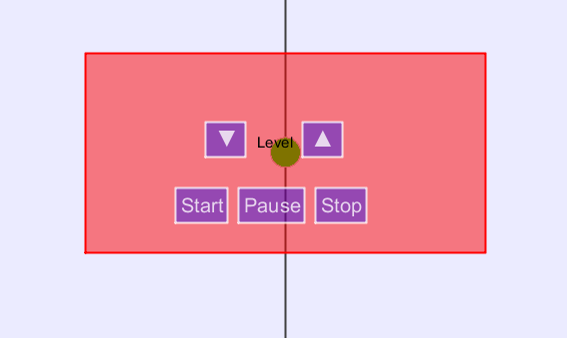
\includegraphics{../img/pong.png}
\end{center}

\end{multicols}

